\documentclass[11pt]{article}

\usepackage[margin=1in]{geometry}
\usepackage{booktabs}
\usepackage{graphicx}
\usepackage{amsmath}
\usepackage{amssymb}
\usepackage{hyperref}

\hypersetup{colorlinks=true, linkcolor=blue, urlcolor=blue}

\newcommand{\sep}{\texttt{x}}
\newcommand{\subj}[1]{\texttt{a\_#1}}
\newcommand{\obj}[1]{\texttt{b\_#1}}
\newcommand{\rel}[1]{\texttt{r\_#1}}
\newcommand{\fatt}[1]{\texttt{f\_#1}}
\newcommand{\gatt}[1]{\texttt{g\_#1}}
\newcommand{\Rsem}{R_{\mathrm{sem}}}
\newcommand{\Rrnd}{R_{\mathrm{rnd}}}
\providecommand{\enote}[2]{}

\title{Goal 1: An Infrequent Semantic Relation Learns a Shared Affine Representation Through a Nonlinear Lookup}
\author{factual-recall-mechanisms}
\date{2026-08-19}

\begin{document}
\maketitle

\section{Result}

We train a small transformer for one epoch on a synthetic corpus containing a
semantic relation $\Rsem$ and a frequency-matched random control $\Rrnd$.  At
\enote{hs}{``exactly one epoch'' is completely vacuous?}
$F{=}16$ occurrences per triple, $\Rsem$ reaches recall $0.672$ on trained triples
and $0.635$ on subjects absent from all relation triples.  An ordinary least-squares
map from subject embeddings to object embeddings also selects the correct held-out
object with accuracy $0.990\pm0.007$ across three seeds; chance is $0.03$.
\enote{hs}{but the important question is whether the object of a held-out triple
is correctly predicted, not the subject? -- now i understand. nice!}

The representation contains the affine structure.  For the fixed-relation map
from subject residuals to object logits, the affine fit
has $R^2=.965\pm.010$ and relative error $.185\pm.027$.  The same map has midpoint
defect $.352\pm.011$ and exact-Jacobian dispersion $.281\pm.013$, both nonzero.
The executed lookup is therefore nonlinear and not J-equivalent on the tested
domain.  Attribute training creates the shared affine geometry even at $F{=}1$,
well before the transformer recalls the relation reliably.

\section{Data}

\paragraph{Vocabulary (265 tokens).}
A separator \sep; two relation tokens \rel{0}, \rel{1}; 192 subject tokens $\subj{0},\dots,\subj{191}$; 32 object tokens $\obj{0},\dots,\obj{31}$; 32 attribute tokens $\fatt{0},\dots,\fatt{31}$; 6 attribute tokens $\gatt{0},\dots,\gatt{5}$.

\paragraph{Entities and attributes.}
Subject $\subj{i}$ has attribute pair
\[
  (f_{i \bmod 32},\ g_{\lfloor i/32\rfloor}).
\]
The 192 subjects cover each of the $32\times6$ combinations once.  Object
$\obj{j}$ has attribute pair
\[
  (f_{(j+3) \bmod 32},\ g_0).
\]

\paragraph{Sentences.}
All training sentences have five tokens:
\begin{center}
\begin{tabular}{ll}
attribute sentence & \sep\ $\subj{i}$\ \fatt{p}\ \gatt{q}\ \sep \quad and \quad \sep\ $\obj{j}$\ \fatt{p}\ \gatt{q}\ \sep\\
relation triple & \sep\ $\subj{i}$\ $\rel{r}$\ $\obj{t}$\ \sep
\end{tabular}
\end{center}

\paragraph{Relations.}
\[
\Rsem(a_i) = b_{f(i)}, \qquad \Rrnd(a_i) = b_{\rho(i)},
\]
Here $f(i) = i \bmod 32$ is the subject's $f$-attribute index.  The semantic
target is the object whose shifted $f$-attribute matches that index.  The function
$\rho$ is a seed-dependent balanced random assignment to the same 32 objects and
is independent of the attributes.  For example, in seed 19, \subj{37} has
attributes $(\fatt{5}, \gatt{1})$.  Its semantic target is \obj{5}, whose attribute
sentence reads \sep\ \obj{5}\ \fatt{8}\ \gatt{0}\ \sep, while its random target
is \obj{27}.  The corresponding relation sentences are \sep\ \subj{37}\ \rel{0}
\ \obj{5}\ \sep\ and \sep\ \subj{37}\ \rel{1}\ \obj{27}\ \sep.

\paragraph{Split and exact frequency matching.}
For each \fatt-value, four of its six subjects enter relation training and two are
held out.  This gives 128 trained and 64 held-out subjects, with a seed-dependent
split.  The random assignment $\rho$ is balanced within both groups.  Under either
relation, every trained subject occurs in one triple, and every object is the target
of four trained subjects and two held-out subjects.  Each relation contributes 128
training triples, repeated $F$ times.  The relations therefore have identical
frequency statistics.  Held-out subjects occur in attribute sentences but in no
relation triple.  The test \texttt{tests/test\_linear\_shift.py} checks these
invariants.

\section{Model and training}

\begin{center}
\begin{tabular}{ll}
\toprule
Model & causal transformer, 1 layer, hidden 64, 4 heads, context 8\\
Embeddings & input and output embeddings untied; all weights $\mathcal{N}(0, 0.02^2)$\\
 & \textbf{no} attribute-based initialization; nothing frozen; no loss reweighting\\
Parameters & 84{,}288\\
Corpus & every attribute sentence $\times A{=}128$ ($= 28{,}672$ sentences)\\
 & $+$ 128 triples per relation, each $\times F$ ($F \in \{1,4,16,64\}$)\\
Training & \textbf{exactly one epoch}: a single pass over the shuffled corpus\\
Steps & 452 ($F{=}1$) to 704 ($F{=}64$) steps at batch size 64\\
Objective & unweighted next-token cross-entropy on all positions\\
Optimizer & AdamW, constant LR $10^{-3}$ after 5 linear warmup steps,\\
 & weight decay 0, gradient clip 1.0\\
Seeds & 19, 31, 47 (control data assignment, initialization, and data order)\\
\bottomrule
\end{tabular}
\end{center}

At $F{=}1$ every relation triple occurs exactly once in the entire training history of the model.

\enote{hs}{i didn't understand what steps are}

\section{Metrics}

\paragraph{Shared-rule probe.}
The representation-level diagnostic measures whether one affine rule transfers to
subjects excluded from relation training:

\begin{quote}
Fit $\hat W, \hat b$ by ordinary least-squares linear regression from the subject's \emph{input embedding} $s_i \in \mathbb{R}^{64}$ to the target object's \emph{output embedding} (unembedding row) $o_{R(i)} \in \mathbb{R}^{64}$, using the 128 trained pairs. For each of the 64 held-out subjects, predict $\hat W s_j + \hat b$ and select the nearest object row by cosine similarity among all 32 objects. Report the fraction of held-out subjects for which the selected object is $R(j)$. Chance is $1/32 \approx 0.03$.
\end{quote}

Each subject has one correct object under each relation, so top-$k$ metrics are
unnecessary.  We separately record greedy next-token recall on prompts \sep\
$\subj{i}$\ $\rel{r}$ for trained and held-out subjects.  Recall checks that the
model learned the relation facts.  The OLS probe instead tests whether the subject
and object embedding spaces admit one affine decoder that transfers to unseen
relation subjects.  It measures representation geometry and generalization; it
does not classify the transformer's computation as affine.

\paragraph{Transformation-level affine and J-equivalence tests.}
For a fixed relation token, each learned sublayer defines a continuous map on its
residual-stream coordinates.  We test six maps: normalized subject state to
attention update; subject residual to post-attention residual; normalized
post-attention state to MLP update; post-attention residual to post-MLP residual;
post-MLP residual to centered object logits; and subject residual to centered
object logits.  These are the attention core, attention block, MLP core, MLP block,
readout, and full lookup.

For each map, we report a four-fold target-stratified affine reconstruction on the
128 trained subjects, normalized midpoint defect, and dispersion of exact
Jacobians across subjects.  An affine map has zero midpoint defect and a constant
Jacobian.  We also report decision accuracy after replacing the map output with its
affine prediction, but this substitution does not prove affinity.  On a synthetic
affine control, the implementation gives midpoint defect below $10^{-6}$ and
Jacobian dispersion below $10^{-12}$.

\section{Results}

\begin{table}[ht]
\centering
\begin{tabular}{rcccccc}
\toprule
 & \multicolumn{2}{c}{probe accuracy (held-out)} & \multicolumn{2}{c}{recall (trained)} & \multicolumn{2}{c}{recall (held-out)}\\
$F$ & $\Rsem$ & $\Rrnd$ & $\Rsem$ & $\Rrnd$ & $\Rsem$ & $\Rrnd$\\
\midrule
1  & $1.000 \pm .000$ & $.031 \pm .013$ & .029 & .010 & .016 & .010\\
4  & $1.000 \pm .000$ & $.016 \pm .013$ & .055 & .034 & .057 & .031\\
\textbf{16} & $\mathbf{0.990 \pm .007}$ & $.036 \pm .007$ & \textbf{.672} & .167 & \textbf{.635} & .031\\
\midrule
control: no triples & $1.000 \pm .000$ & $.021 \pm .015$ & -- & -- & .000 & .000\\
\bottomrule
\end{tabular}
\caption{Low-frequency results, reported as mean $\pm$ sd over seeds 19/31/47 at
$A{=}128$.  The value $F$ is the number of occurrences of each of the 128 triples
per relation.  At $F{=}16$, $\Rsem$ reaches recall .672 on trained subjects and
.635 on held-out subjects, while its affine embedding decoder transfers at .990.
The frequency-matched $\Rrnd$ is barely recalled and shows no shared-rule transfer.
The table concerns learning and representation geometry, not the affinity of the
executed transformation.}
\label{tab:goal1}
\end{table}

\begin{figure}[ht]
\centering
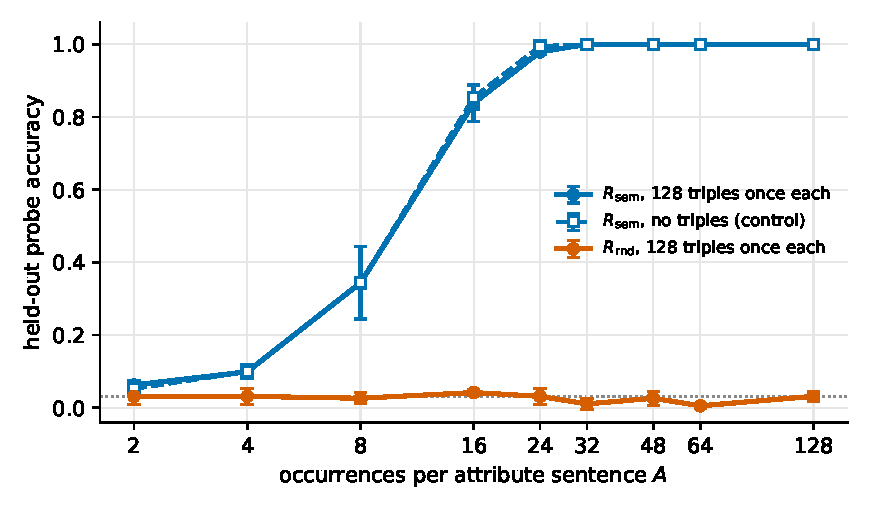
\includegraphics[width=0.72\textwidth]{figures/linear_shift_transition.pdf}
\caption{Held-out shared-rule probe accuracy at $F{=}1$ as attribute-sentence
frequency $A$ increases.  Every relation triple occurs once in the solid curve;
the dashed control contains no relation triples.  Both curves undergo the same
transition from chance to affine decodability.  The random relation has no
transferable counterpart.}
\label{fig:transition}
\end{figure}

\paragraph{Low-frequency relation learning ($F{=}16$).}
With each fact occurring 16 times in one epoch, $\Rsem$ reaches recall $.672$ on
trained triples and $.635$ on held-out subjects.  The embedding probe transfers at
$0.990$.  The frequency-matched random control reaches only $.167$ recall and its
probe stays at chance.  Shared attribute geometry lets the semantic relation learn
and generalize earlier.  These measurements concern structure and transfer.

\paragraph{Affine geometry after one occurrence ($F{=}1$).}
At $F{=}1$, the probe is already $1.000$ for $\Rsem$ and remains at chance for
$\Rrnd$.  The model still fails to recall individual triples at this point
($\approx .03$), so this is a representation result rather than a behavioral one.

\paragraph{Attribute training drives the decodability transition.}
At $F{=}1$, increasing the attribute-sentence frequency changes the $\Rsem$ probe
from $0.05$ to $0.10$, $0.34$, $0.85$, and $1.00$ for
$A=2,4,8,16,24$ (Fig.~\ref{fig:transition}).  The zero-triple control follows the
same curve.  Attribute sentences therefore build the affine subject-to-object
geometry.  The single-occurrence semantic triples agree with that geometry, and
the model uses it once recall emerges.

\begin{table}[ht]
\centering
\small
\begin{tabular}{lccccc}
\toprule
Map & affine $R^2$ & rel. error & affine decision & midpoint defect & Jacobian disp.\\
\midrule
attention core & $.993\pm.002$ & $.080\pm.012$ & $.742\pm.072$ & $.035\pm.007$ & $.085\pm.013$\\
attention block & $.983\pm.004$ & $.129\pm.015$ & $.750\pm.066$ & $.273\pm.010$ & $.179\pm.005$\\
MLP core & $.983\pm.003$ & $.131\pm.011$ & $.742\pm.061$ & $.095\pm.005$ & $.137\pm.007$\\
MLP block & $.974\pm.006$ & $.160\pm.017$ & $.758\pm.057$ & $.247\pm.027$ & $.172\pm.009$\\
readout & $.993\pm.003$ & $.081\pm.017$ & $.760\pm.060$ & $.199\pm.004$ & $.228\pm.007$\\
full lookup & $.965\pm.010$ & $.185\pm.027$ & $.750\pm.056$ & $.352\pm.011$ & $.281\pm.013$\\
\bottomrule
\end{tabular}
\caption{Transformation tests for $\Rsem$ at $F{=}16$.  Affine fits use four
target-stratified folds, so every trained subject is evaluated once.  An affine or
J-equivalent map would have zero midpoint defect and zero Jacobian dispersion.  All
six maps are nonlinear by these tests, although the quality of their affine
approximations differs.}
\label{tab:goal1-transformation}
\end{table}

\paragraph{The semantic lookup is nonlinear.}
The full lookup has midpoint defect $.352\pm.011$ and exact-Jacobian dispersion
$.281\pm.013$.  Dispersion remains $.284\pm.013$ on the empirical
subject-difference subspace, ruling out an explanation based only on off-manifold
directions.  The high affine $R^2$ and transferred embedding decoder show a close
affine approximation.  The nonzero defects show that the trained transformer is
neither affine nor J-equivalent on the tested domain.

\section{Learned representation and causal mechanism}

Attribute training organizes the subject embeddings into 32 code families, one
for each $f(i)$ value, instead of storing the 128 semantic triples independently.
A target-class centroid learned from the 128 trained subjects classifies the
embeddings of the 64 held-out relation subjects with accuracy $1.000\pm.000$.
The class remains decodable from concatenated attention-head outputs at
$1.000\pm.000$, from the post-attention state at $.990\pm.007$, and from the final
state at $.990\pm.007$.  The model represents $f(i)$ as a distributed direction in
the subject embedding.  Subjects with the same $f$ value share that task-relevant
component while retaining identity and $g$ information.

Each object has a learned output-embedding direction.  The relation-conditioned
MLP and output readout convert the transported $f$-class code to the corresponding
object direction.  The pseudocode below records the causal information flow.  It
does not assume that the component maps are affine.

\begin{small}
\begin{verbatim}
def answer_semantic(subject):
    # Learned representation: a shared code for f(subject).
    subject_code = embedding[subject]

    # H3 and H1 carry most of the subject's value payload;
    # H0/H2 provide smaller, seed-dependent support.
    payload = sum(head[h].read_value(subject_code, relation=r0)
                  for h in [H0, H1, H2, H3])

    # r0 selects the shared class-to-object readout.
    state = relation_state[r0] + project(payload)
    state += distributed_class_readout(state)
    object_scores = dot(final_normalize(state), object_directions)
    return argmax(object_scores)          # b[f(subject)]
\end{verbatim}
\end{small}

In the pseudocode, \texttt{read\_value} multiplies the subject's projected value by
the attention weight assigned to that subject.  Separator and relation
contributions do not change under a subject swap and belong to the baseline.  The
final \texttt{dot} compares the resulting state with 32 learned object-output
directions.

The interventions locate the information in the value payload.  Swapping that
payload between two subjects restores $.987\pm.008$ of the corresponding change in
the correct-object logit; swapping only their attention weights restores
$.013\pm.007$.  A swap of all head outputs restores the full effect.  Replacing
every head output with its training-subject mean reduces object accuracy from
$.729\pm.094$ to chance ($.031\pm.000$).  The downstream computation therefore
uses the class code detected by the probes.

The relation token selects how the model interprets the transported subject code.
When the subject is fixed and $\rel{0}$ is exchanged with $\rel{1}$, a head-output
patch restores $.070\pm.007$ of the relation effect, while an MLP-population patch
restores $.850\pm.017$.  The heads primarily move subject content; the $\rel{0}$
residual selects the semantic readout downstream.

The final conversion is distributed across the MLP.  Keeping only the 32 units
with the largest causal effects recovers $.498\pm.029$ of the subject-specific
margin.  Ablating those units still leaves $.790\pm.032$, so no small group carries
the computation alone.  An affine surrogate for every GELU preserves held-out
object accuracy ($.729\pm.092$ versus $.729\pm.094$) and explains $.962\pm.001$ of
activation variance.  This intervention provides an accurate approximation and
preserves the decisions, but it does not reproduce the MLP transformation exactly.
\enote{hs}{affine replacement of gelus: interesting. discuss}
The MLP core has midpoint defect $.095\pm.005$ and Jacobian dispersion
$.137\pm.007$; the full MLP block gives $.247\pm.027$ and $.172\pm.009$.  Both maps
are nonlinear under the affine/Jacobian definition.

\begin{figure}[ht]
\centering
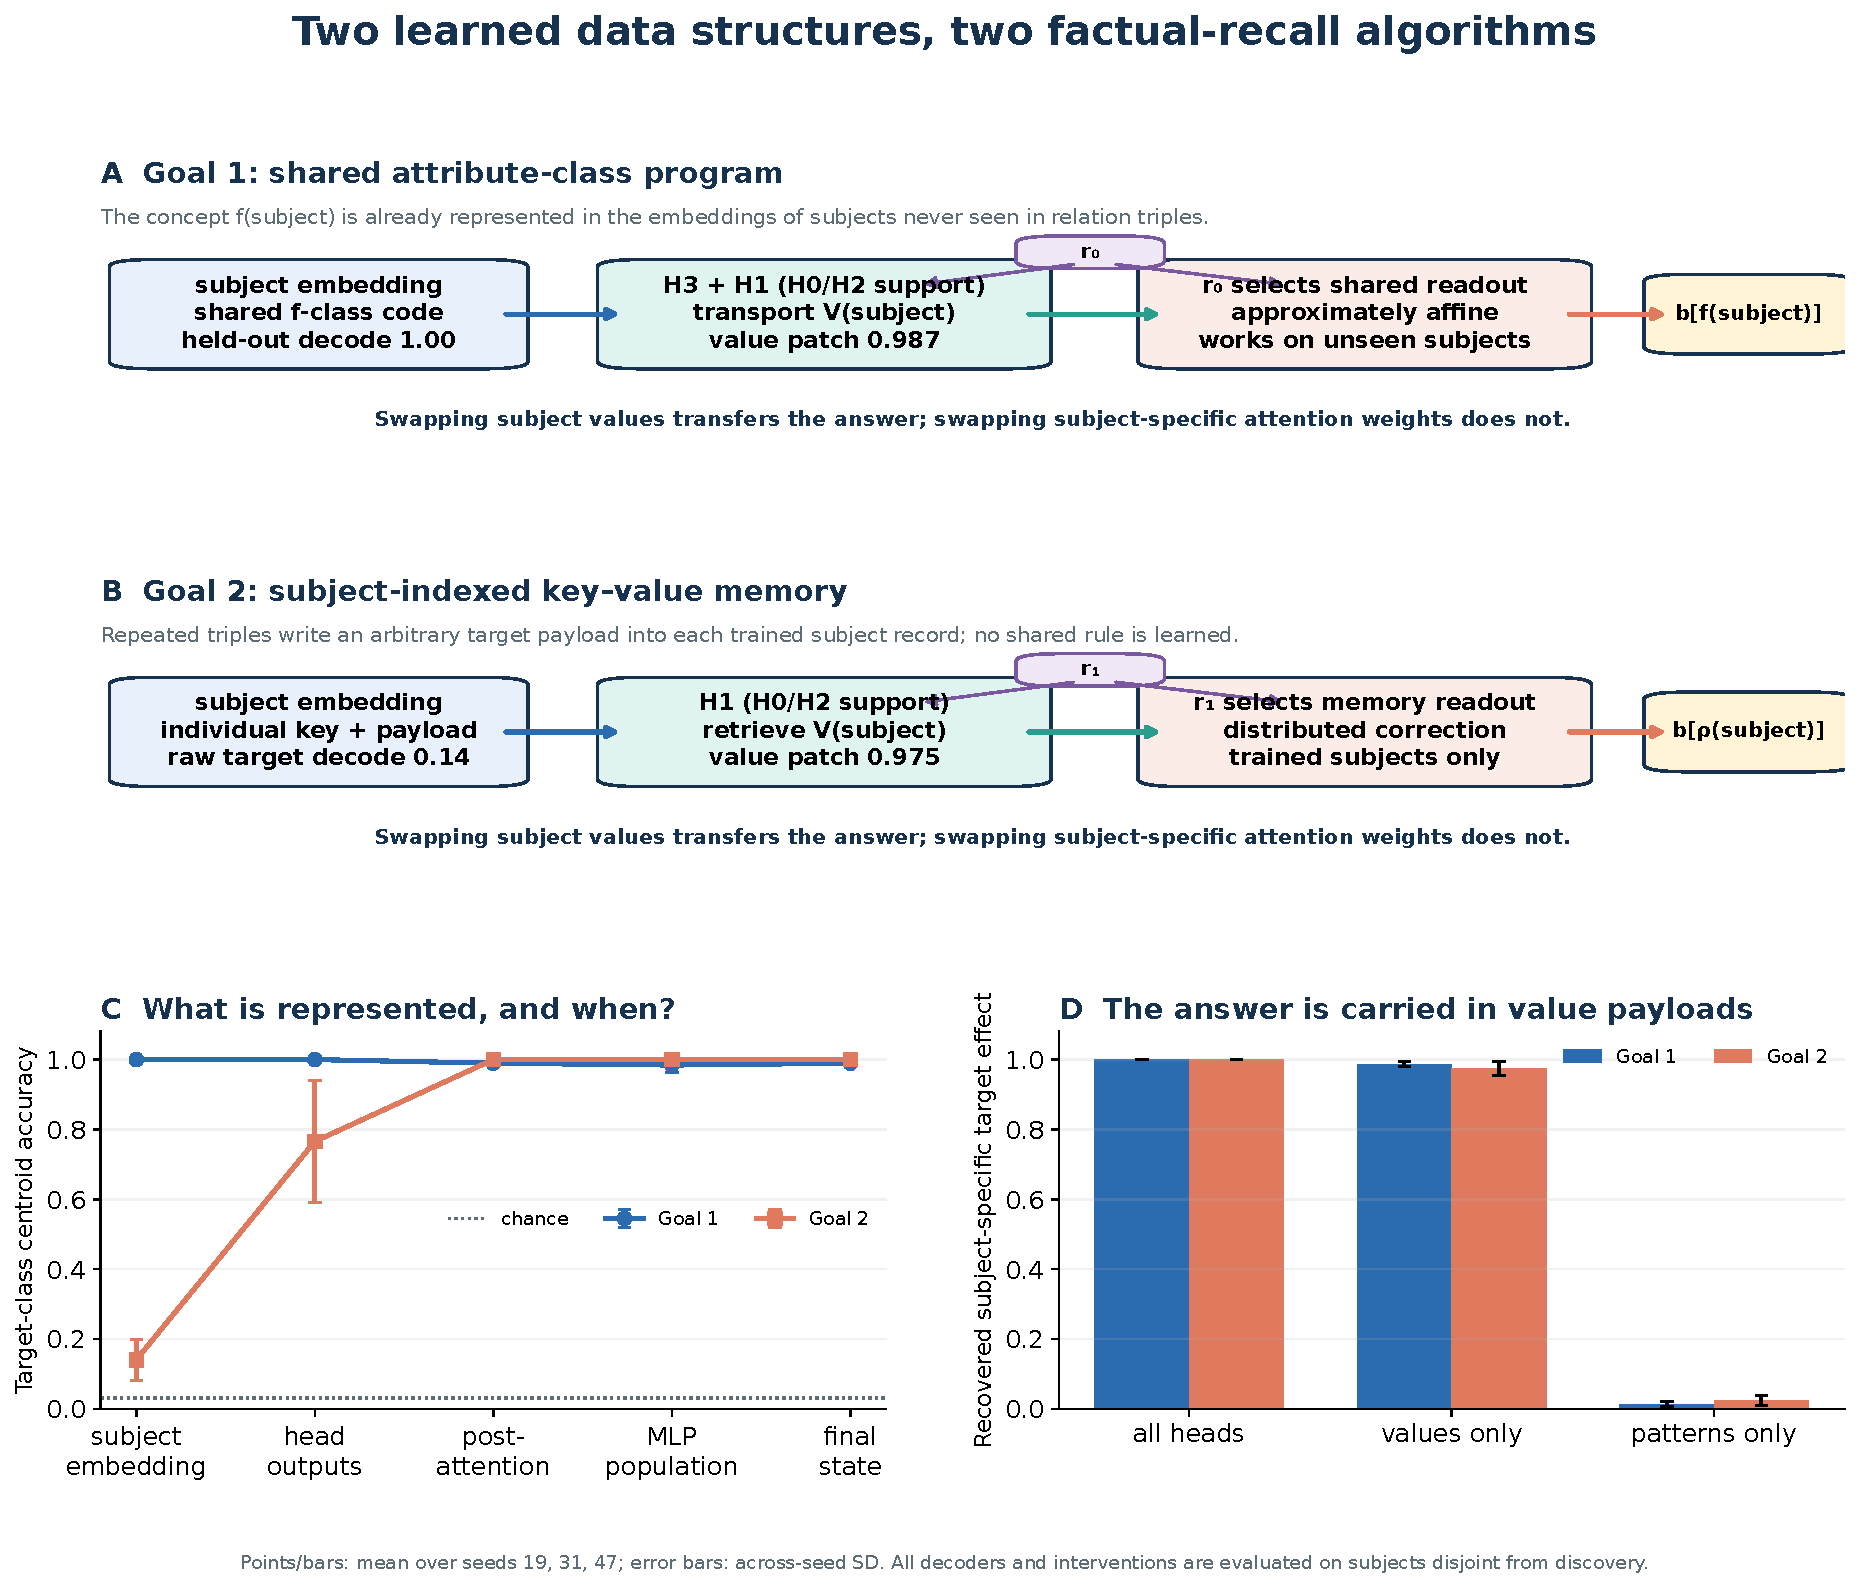
\includegraphics[width=\textwidth]{../factual_recall/results/final_mechanistic_analysis/goal1_goal2_mechanisms.pdf}
\caption{Learned representations and causal information flow in the original
transformer experiments.  For Goal~1, the model transports a shared $f$-class code
to a distributed class-to-object readout.  The lower panels track target
decodability and compare the causal effects of attention values and attention
weights.}
\label{fig:goal12mechanism}
\end{figure}

The probes and interventions support one account of generalization.  Held-out
subject embeddings contain the shared $f$-organized code; the attention value
paths transport it; and a distributed nonlinear MLP/readout converts it to the
correct object direction.  On these prompts, an affine model closely approximates
that computation without matching it exactly.

\section{Scope}

At $F{=}16$, the semantic relation generalizes through a shared,
affine-decodable representation.  Its attention, MLP, readout, and full lookup are
neither affine nor J-equivalent on the tested domain.  The semantic lookup is more
closely approximated by an affine map than the frequency-matched random lookup,
and affine GELU substitution preserves its decisions.  Approximation, decision
equivalence, and exact affinity remain separate properties.

The relation triples do not cause the decodability transition at $F{=}1$.  The
dashed control in Fig.~\ref{fig:transition} attributes that transition to exposure
to attribute sentences.  We also tested three designs in which transfer could only
come from triple-driven structure: a one-to-one relation with separate output rows
for each fact, a conjunction of two attributes with up to $49{,}152$ distinct
facts, and hidden-state probes.  None transferred above chance in the
single-occurrence, one-epoch regime, where each fact contributes one gradient.

Earlier drafts used affine decoding and generalization as the definition of a
linear relation.  Here those measurements support a claim about shared
representation; midpoint and exact-Jacobian tests classify the computation.  The
reported ``single-exposure phase shift'' in those drafts, from $0.27$ to $0.95$,
also disappears under a fixed-size probe and standard initialization.  It arose
because the earlier regression used 10 pairs at the first snapshot and more than
500 later, over embeddings initialized from the attribute geometry.

\end{document}
